\documentclass[12pt]{article}
\usepackage[spanish]{babel}
\usepackage[utf8]{inputenc}
\usepackage[T1]{fontenc}
\usepackage{vmargin}
\usepackage{setspace}
\usepackage{enumerate}
\usepackage{graphicx}
\usepackage{parskip}
\graphicspath{ {images/} }
\usepackage{float} 

\begin{document}
\begin{center}
\includegraphics[scale=0.5]{unison-logo.png}
\\
\vspace{0.5cm}
UNIVERSIDAD DE SONORA \\
\vspace{0.5cm}
DIVISIÓN DE CIENCIAS EXACTAS Y NATURALES \\
\vspace{0.5cm}
DEPARTAMENTO DE FÍSICA\\
\vspace{0.5cm}
LICENCIATURA EN FÍSICA\\
\vspace{0.5cm}
FÍSICA COMPUTACIONAL I

\vspace{2 cm}
\hrule
\vspace{1 cm}

{\huge \bfseries {Teoría del caos y mapeo logístico}}

\vspace{1 cm}
\hrule
\vspace{2 cm}
Martinez López Lizbeth Vanessa \\ 
\vspace{1 cm}
Profesor del curso\\
Dr. Carlos Lizárraga Celaya\\
\vspace{2 cm}
19 de Mayo del 2017
\end{center}
\pagebreak

\begin{doublespace}
\hrule
\section*{Resumen}
En la práctica anterior se habló un poco sobre la teoría del caos, el efecto mariposa y el atractor de Lorenz. En esta práctica seguimos trabajando con la Teoría del caos, siendo el objetivo principal desarrollar diversas gráficas que explican ciertos sistemas caóticos.
\vspace{0.6 cm}
\hrule

\vspace{0.6 cm}

\section{Introducción}

Como ya hemos visto, en la actualidad la teoría del caos es muy famosa. Son muchos los interesados en el estudio de sistemas caóticos, los cuales se apoyan de gráficos que les permitan analizar mejor el comportamiento de dichos sistemas.

En esta práctica veremos algunos ejemplos de gráficas que nos muestran sistemas cuyo comportamiento es caótico. Es Geoff Boeing quien nos presenta un artículo en el cual plasma dichos ejemplos, además de dar una explicación de ellos.

Para el desarrollo de esta actividad se ha utilizado la biblioteca pynamical en Python.

\section{Desarrollo}
Para iniciar esta práctica fue necesario primero instalar pynamical, desde el github de Geoff Boeing se llevó la biblioteca pynamical al github propio, donde fue descargado y guardado en el archivo de la práctica 9. Para instalar la biblioteca se usó el siguiente código: 

\begin{verbatim}
pip install pynamical
\end{verbatim}

Dicho código debe ponerse en el cmd o terminal, la cual debe tener la dirección del archivo de pynamical descargado.

Ya con la biblioteca instalada se procedió a la graficación. El código de los gráficos fue obtenido de la misma biblioteca pynamical, siendo Geoff Boeing de gran ayuda para realizar los gráficos. 

En el código se tuvo que añadir los segmentos de código necesarios para cambiar el color, títulos y leyendas a las gráficas, para ello se hizo uso de las paletas de matplotlib. 

Debido a que son muchas gráficas, se omitirá la presentación del código empleado, sin embargo éste puede verse en los archivos de Python creados.

\section{Resultados}

A continuación se muestran las gráficas en el orden que aparecen en el artículo de Geoff Boeing.

Primero se obtuvo la siguiente tabla:

\begin{center}
\includegraphics[scale=0.6]{1}
\end{center}

En la tabla, las columnas representan tasas de crecimiento y las filas representan generaciones. Geoff explica que el modelo siempre comienza con un nivel de población de 0,5 y se configura para representar la población como una relación entre 0 (extinción) y 1 (la capacidad máxima de carga de nuestro sistema).

El primer gráfico presentado es el siguiente:

\begin{center}
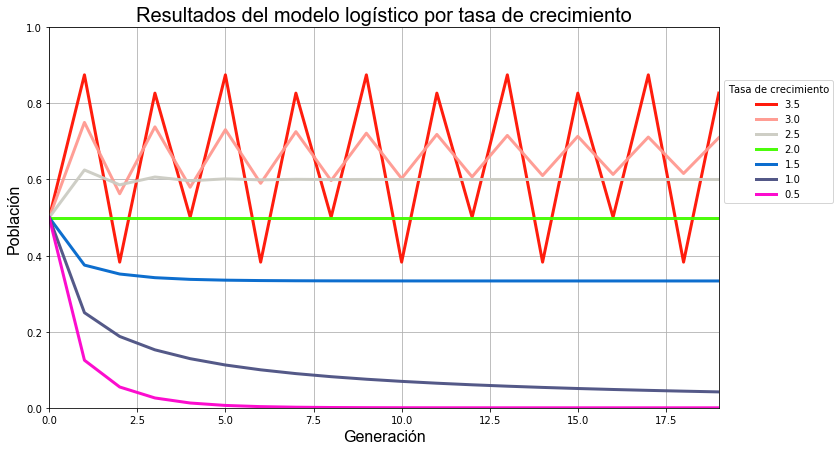
\includegraphics[scale=0.5]{2}
\end{center}

La gráfica es obtenida mediante los datos que se presentan en la tabla anterior. Aquí se puede ver fácilmente cómo la población cambia con el tiempo, dadas las diferentes tasas de crecimiento.

Utilizando los mismos datos de la tabla, se hacen los siguientes diagramas de bifurcación:
\begin{center}
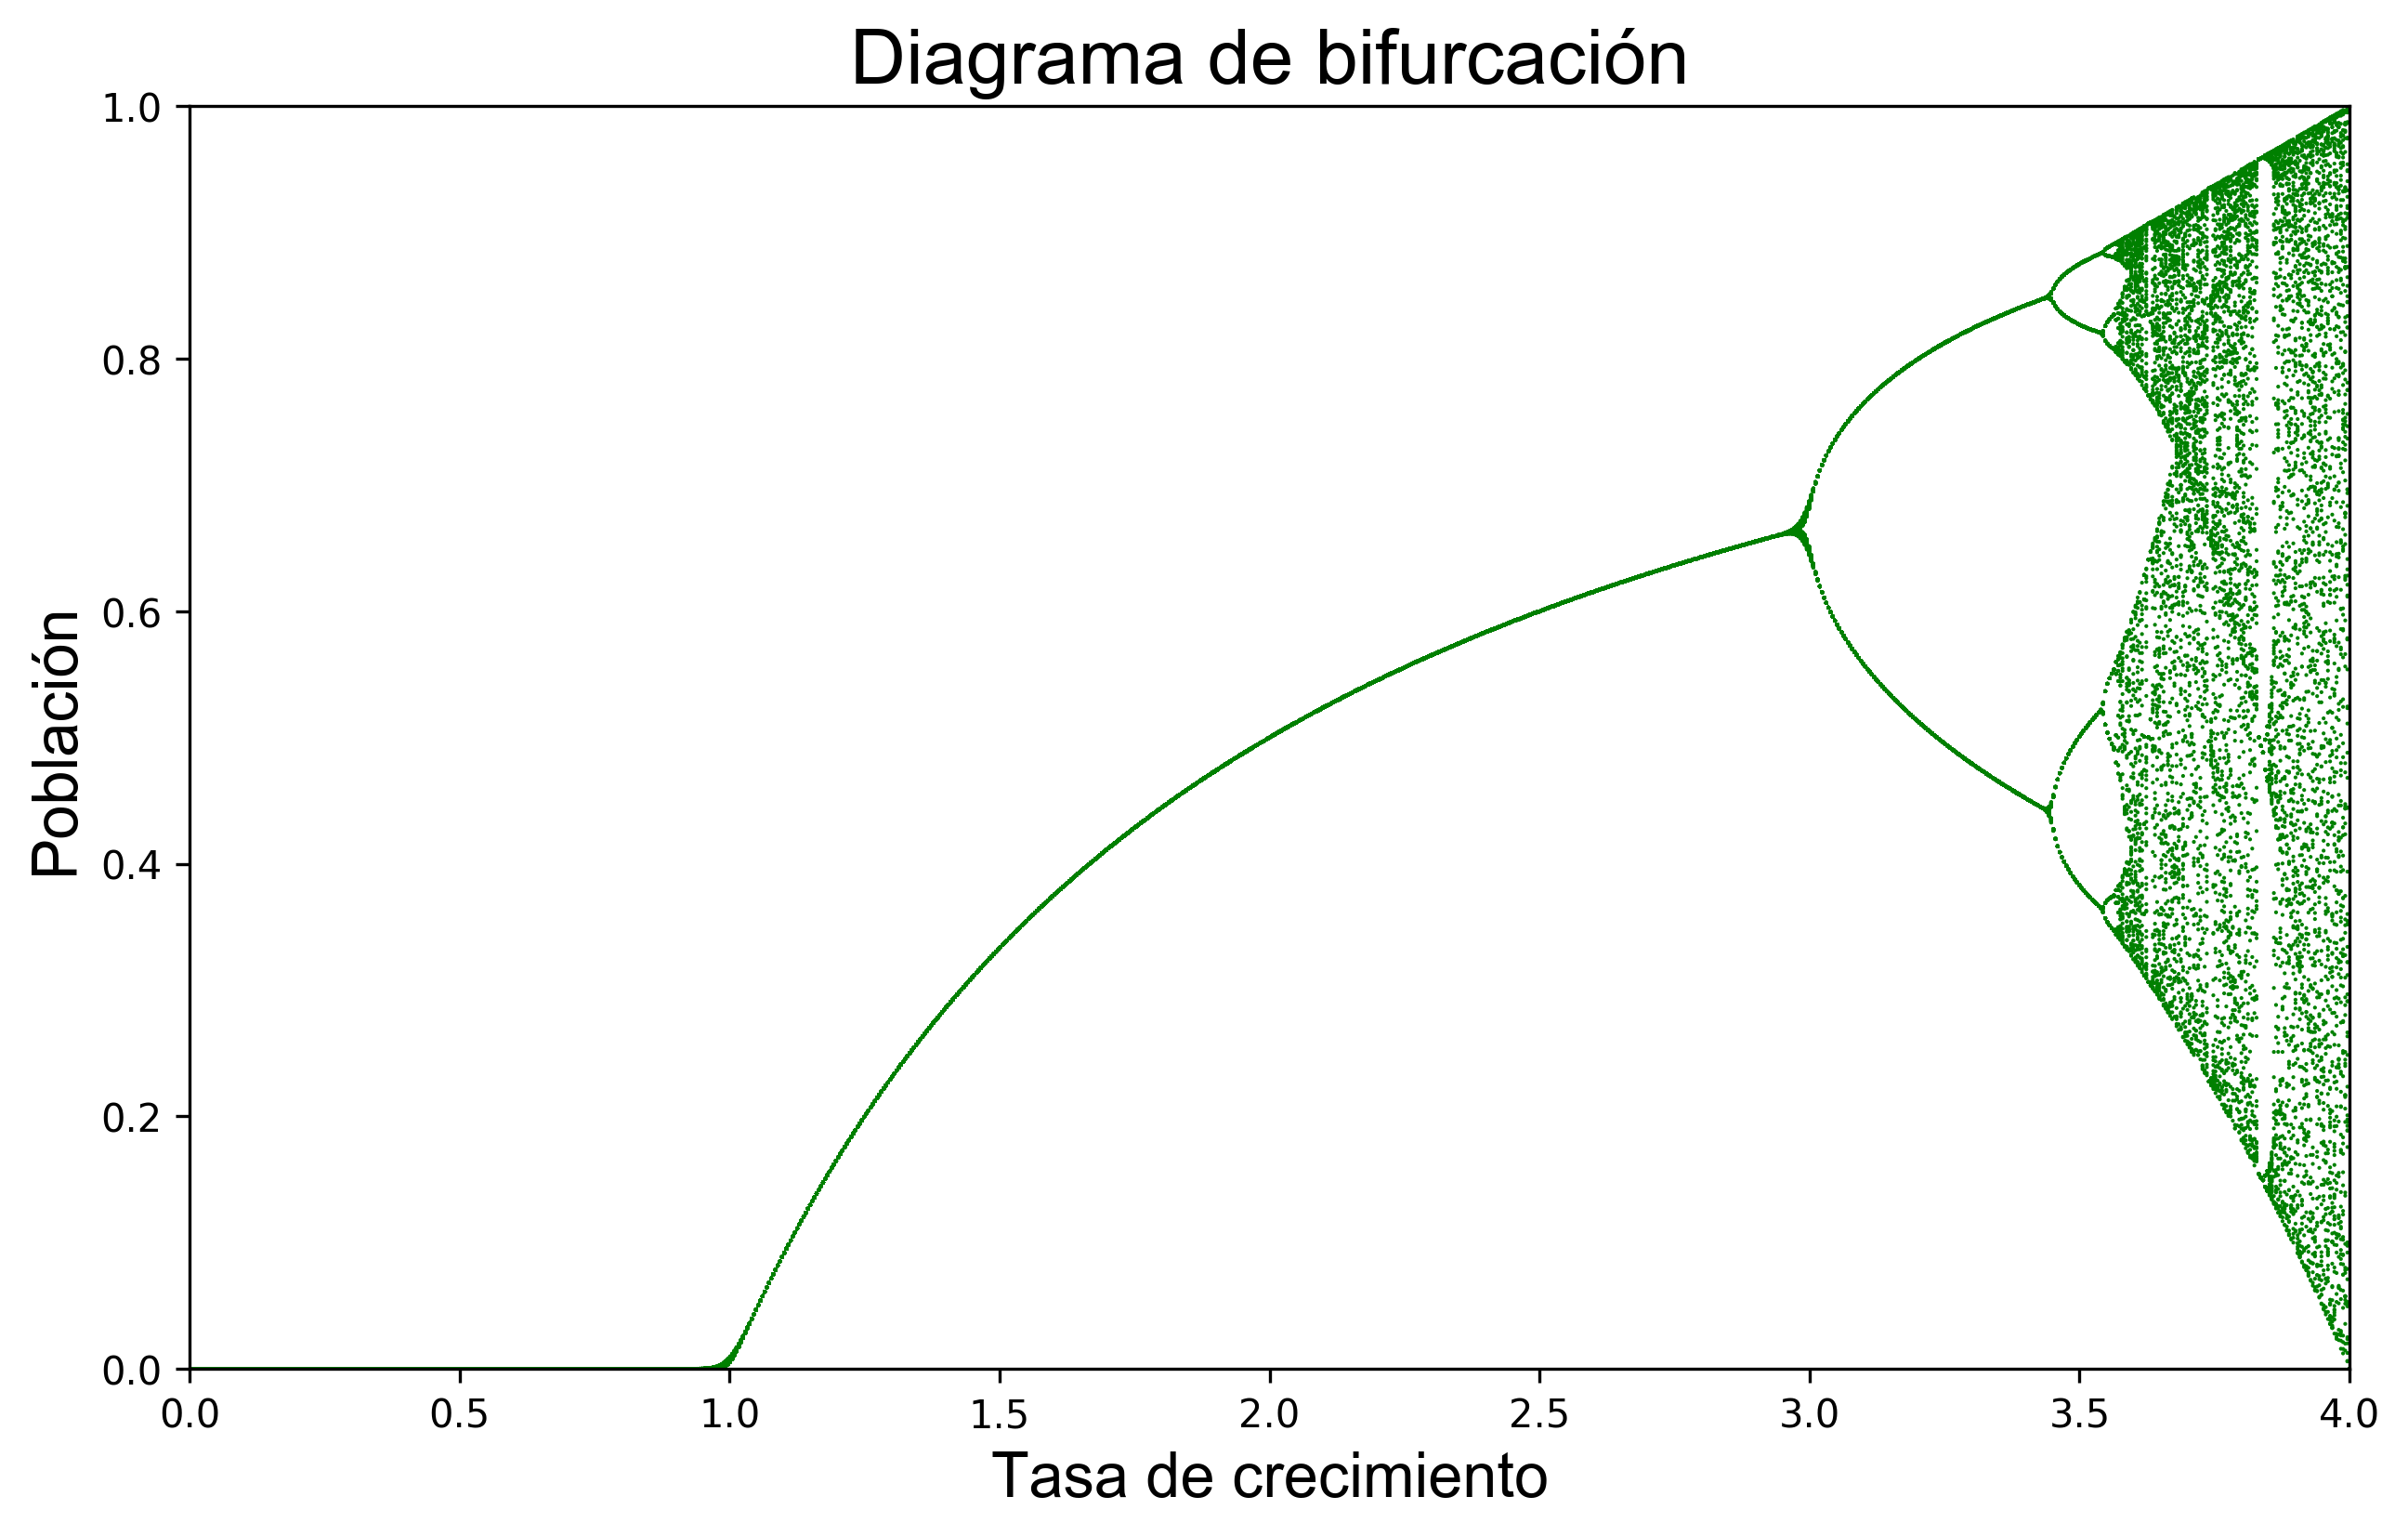
\includegraphics[height=6cm, width=7.5cm]{3}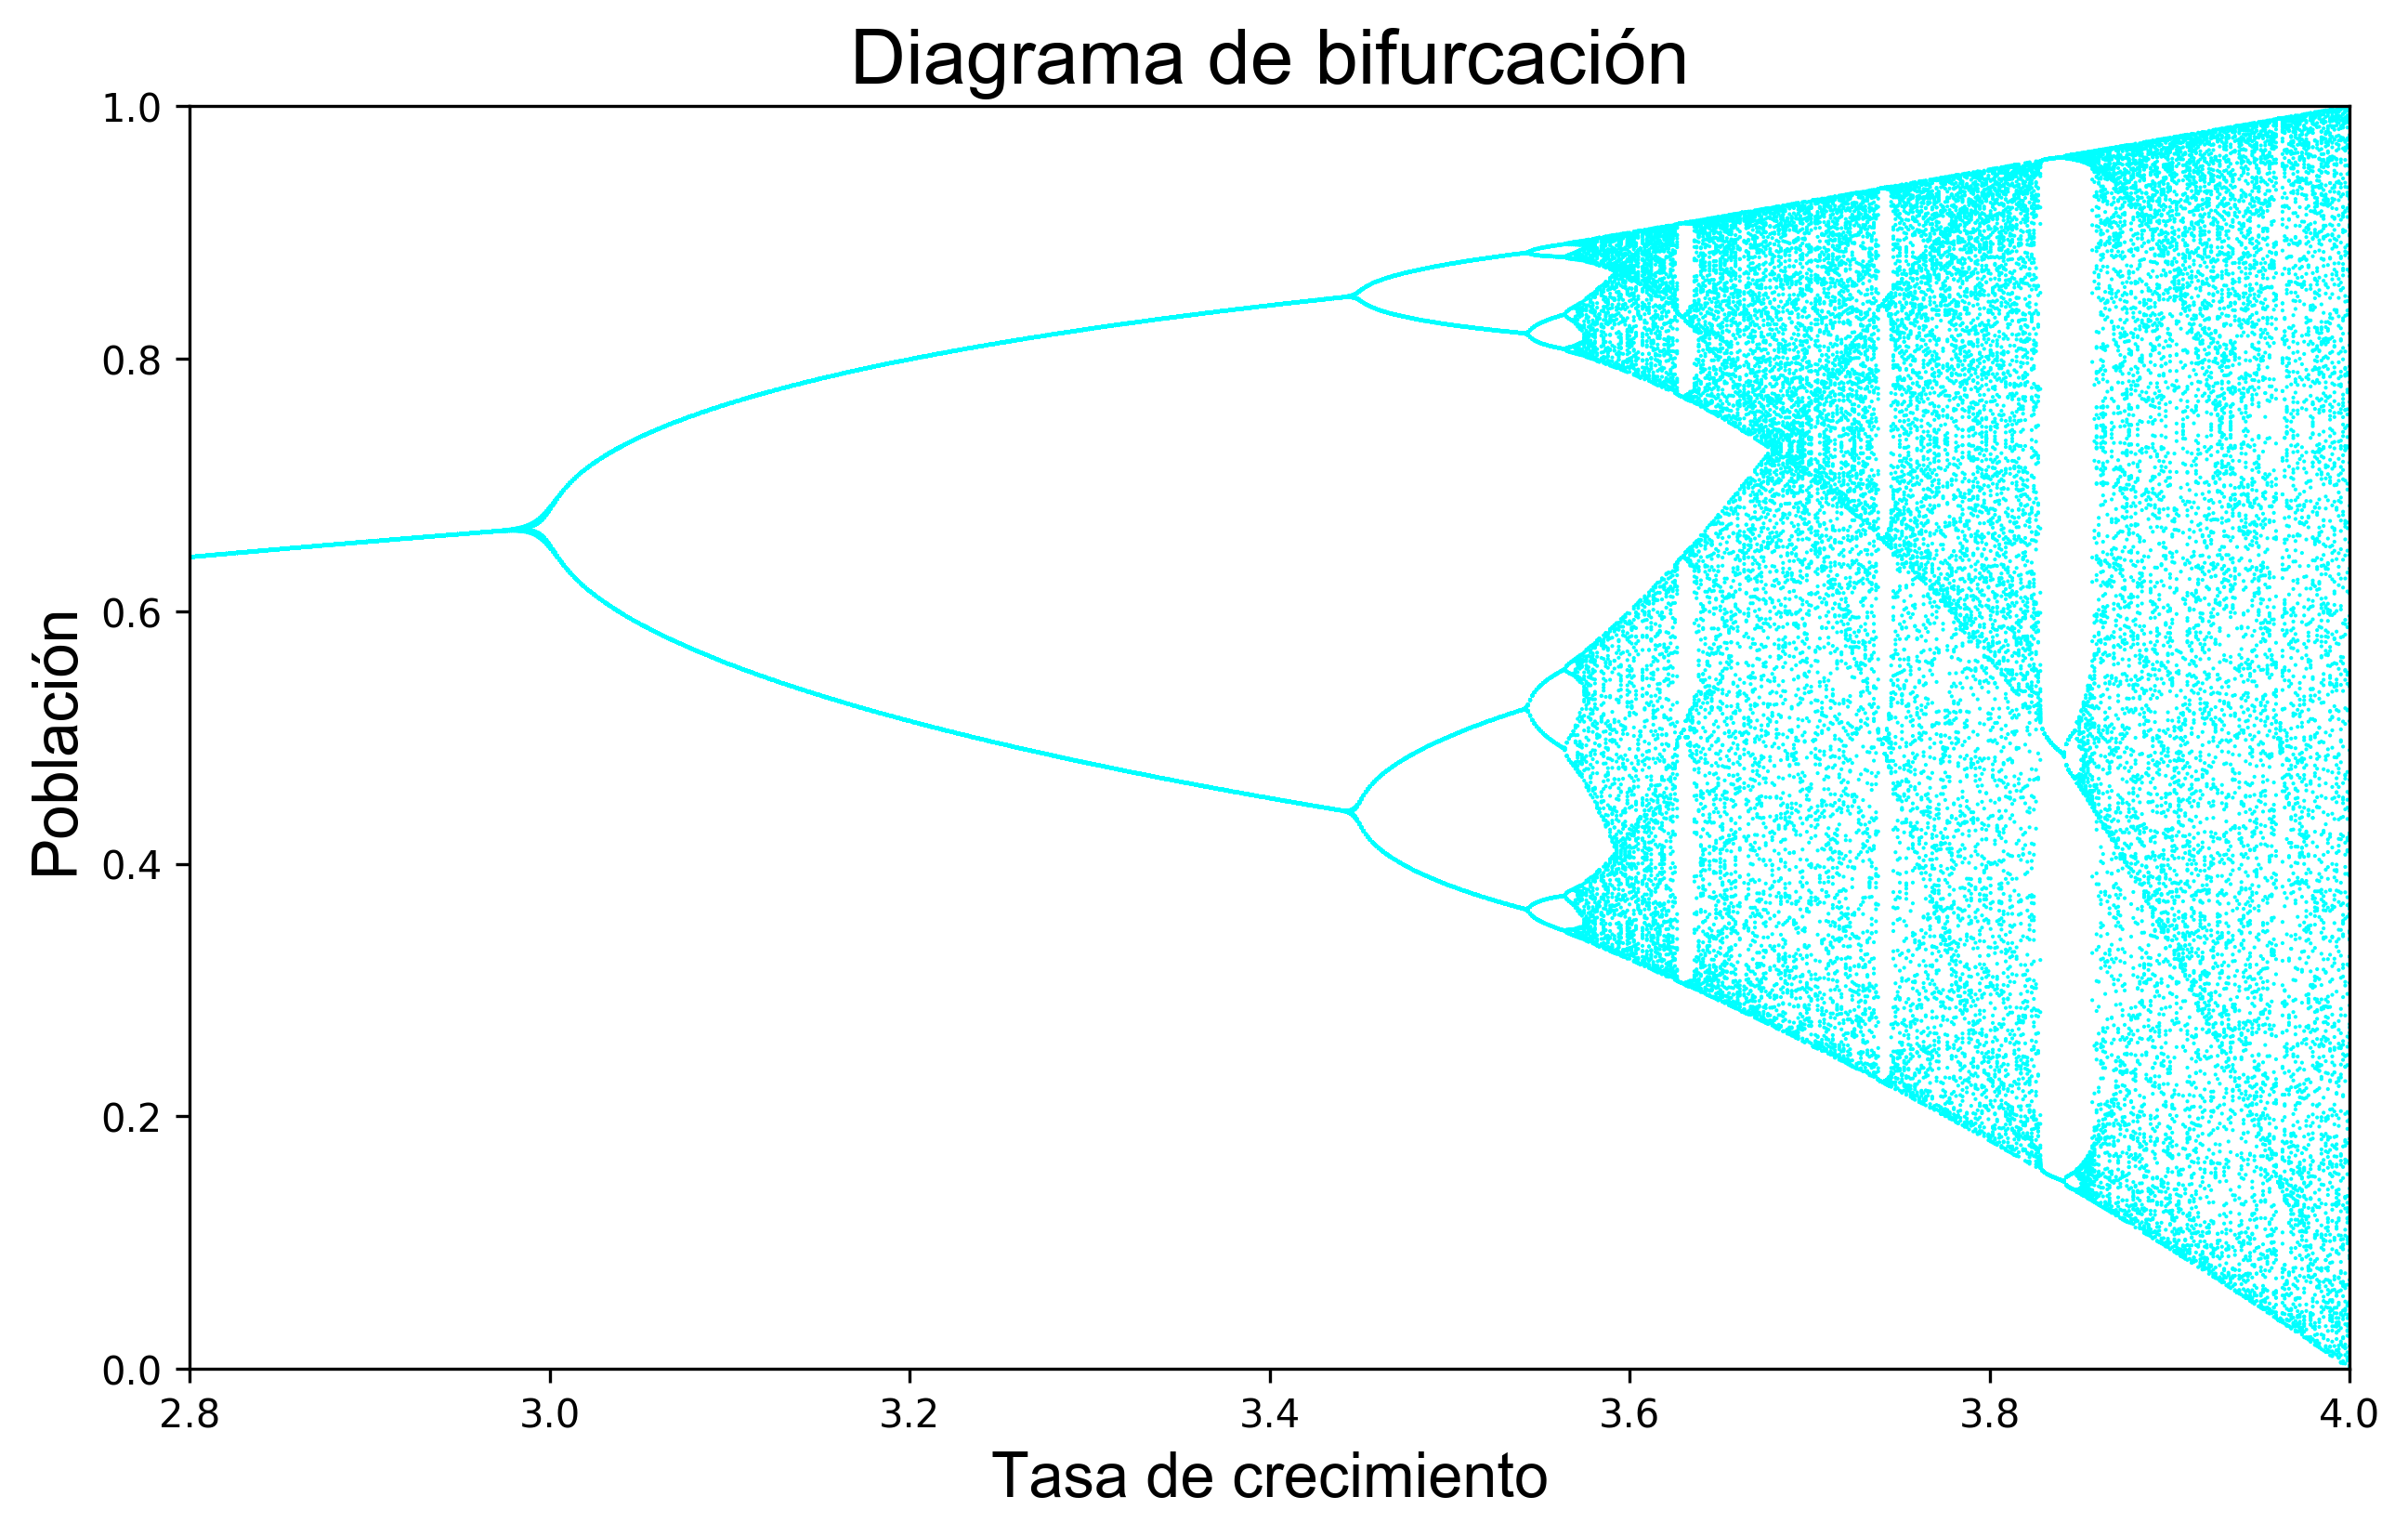
\includegraphics[height=6cm, width=7.5cm]{4}

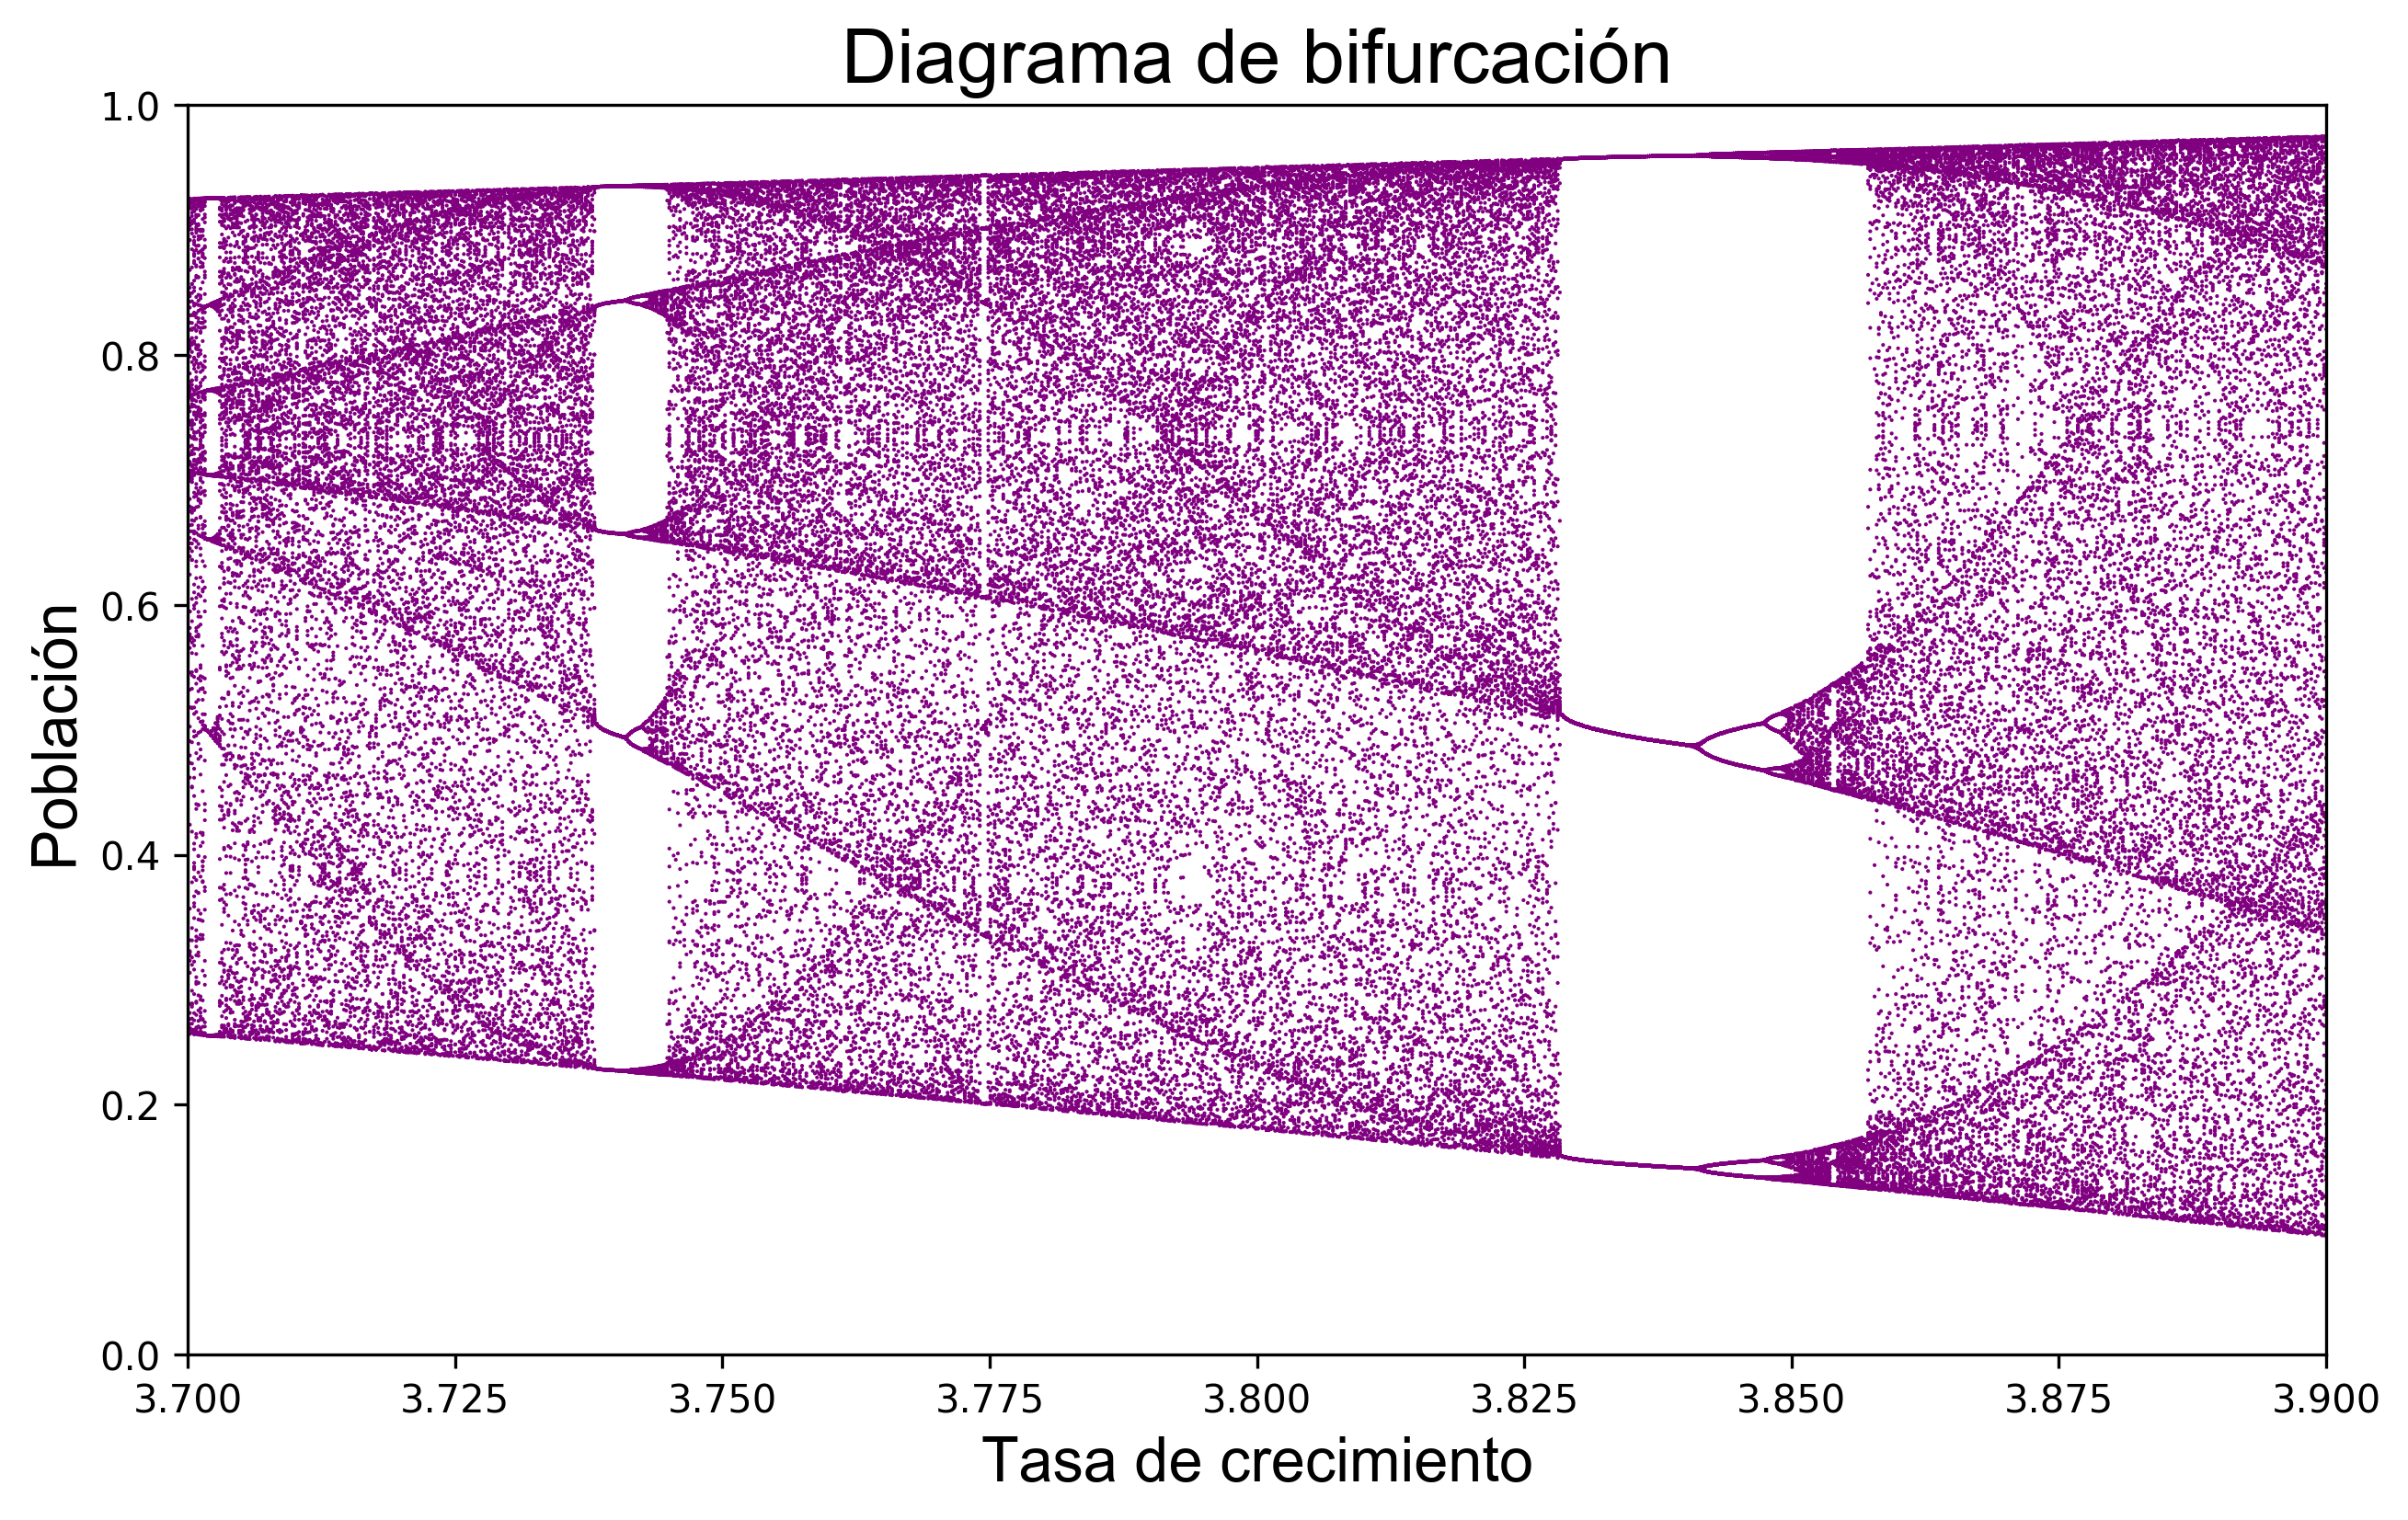
\includegraphics[height=6cm, width=7.5cm]{5}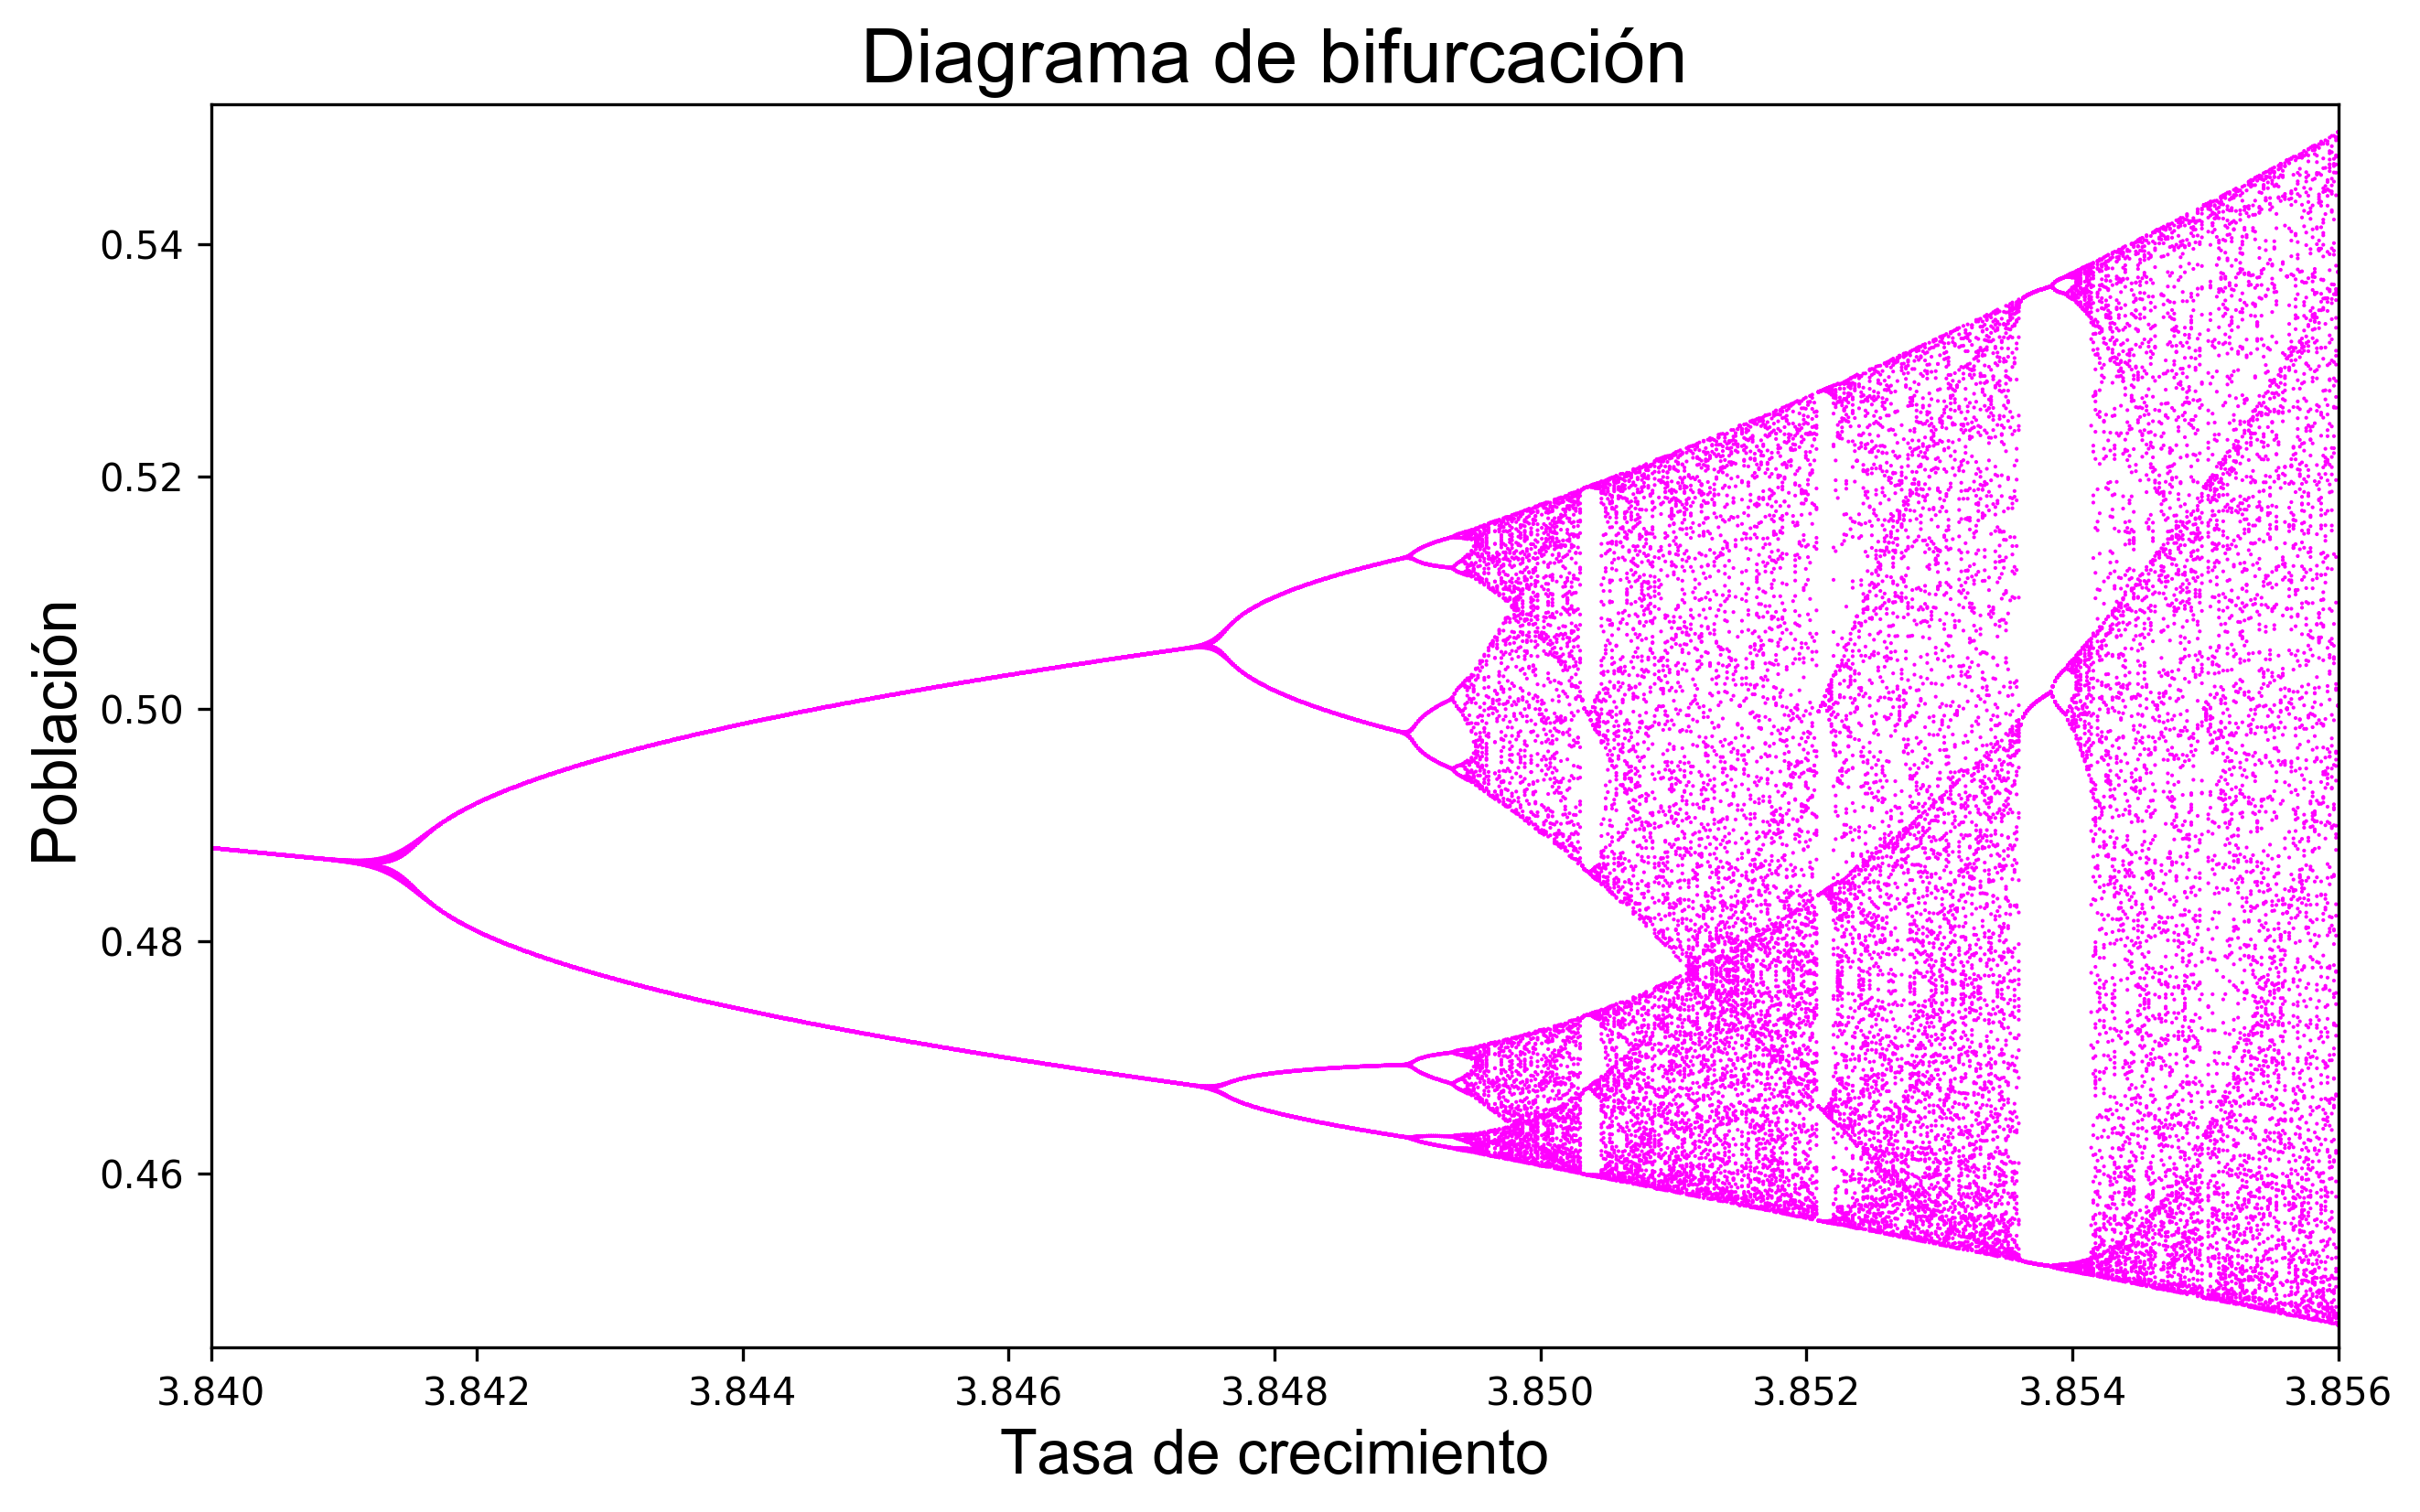
\includegraphics[height=6cm, width=7.5cm]{6}
\end{center}

Para obtener los diagramas de bifurcación, se emplea el modelo logístico cambiando los parámetros, en este caso el modelo logístico se emplea de nuevo, para 200 generaciones a través de 1.000 tasas de crecimiento entre 0.0 a 4.0, esto nos brinda la primer gráfica. Si ampliamos la gráfica en un intervalo de las tasas de crecimiento entre 2,8 y 4,0, obtenemos el segundo diagrama. Se aplica zoom nuevamente en un intervalo de tasas de crecimiento entre 3.7 y 3.9, originando así el tercer diagrama. Para el tercer diagrama, se hace zoom en el centro, en un rango de 3.85. En esta última gráfica, se mira la misma estructura observada en la primera, si se sigue ampliando la imagen infinitamente, se seguirá viendo la misma estructura.

\pagebreak
En las siguientes gráficas, las cuales son diagramas de fases o Gráficas de Poincaré, se muestra lo siguiente: como el modelo que aquí se analiza sigue una regla determinista simple, si se conoce el valor de la población de una determinada generación, se puede determinar fácilmente el valor de la siguiente generación.
\begin{center}
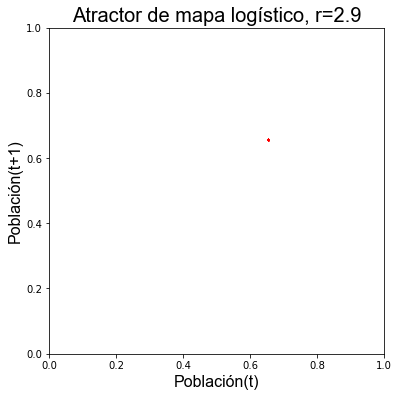
\includegraphics[height=6cm, width=7.5cm]{7}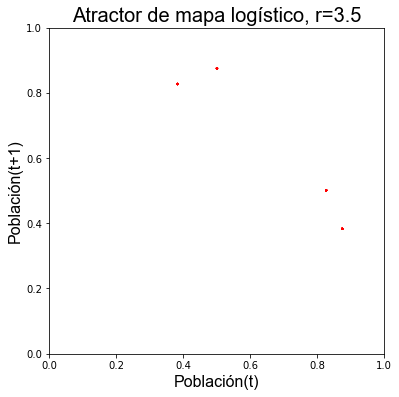
\includegraphics[height=6cm, width=7.5cm]{8}
\end{center}

El diagrama de fases de la izquierda muestra que el mapa logístico se encuentra en un atractor de punto fijo en 0.655 (en ambos ejes) cuando el parámetro de tasa de crecimiento se establece en 2.9. La gráfica de la derecha muestra un atractor de ciclo límite. Cuando la tasa de crecimiento se establece en 3,5, el mapa logístico oscila entre cuatro puntos. 

Esto es lo que sucede cuando estas bifurcaciones de dobles períodos conducen al caos:
\begin{center}
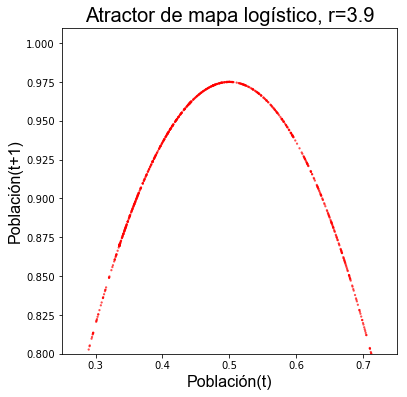
\includegraphics[height=6cm, width=7.5cm]{9}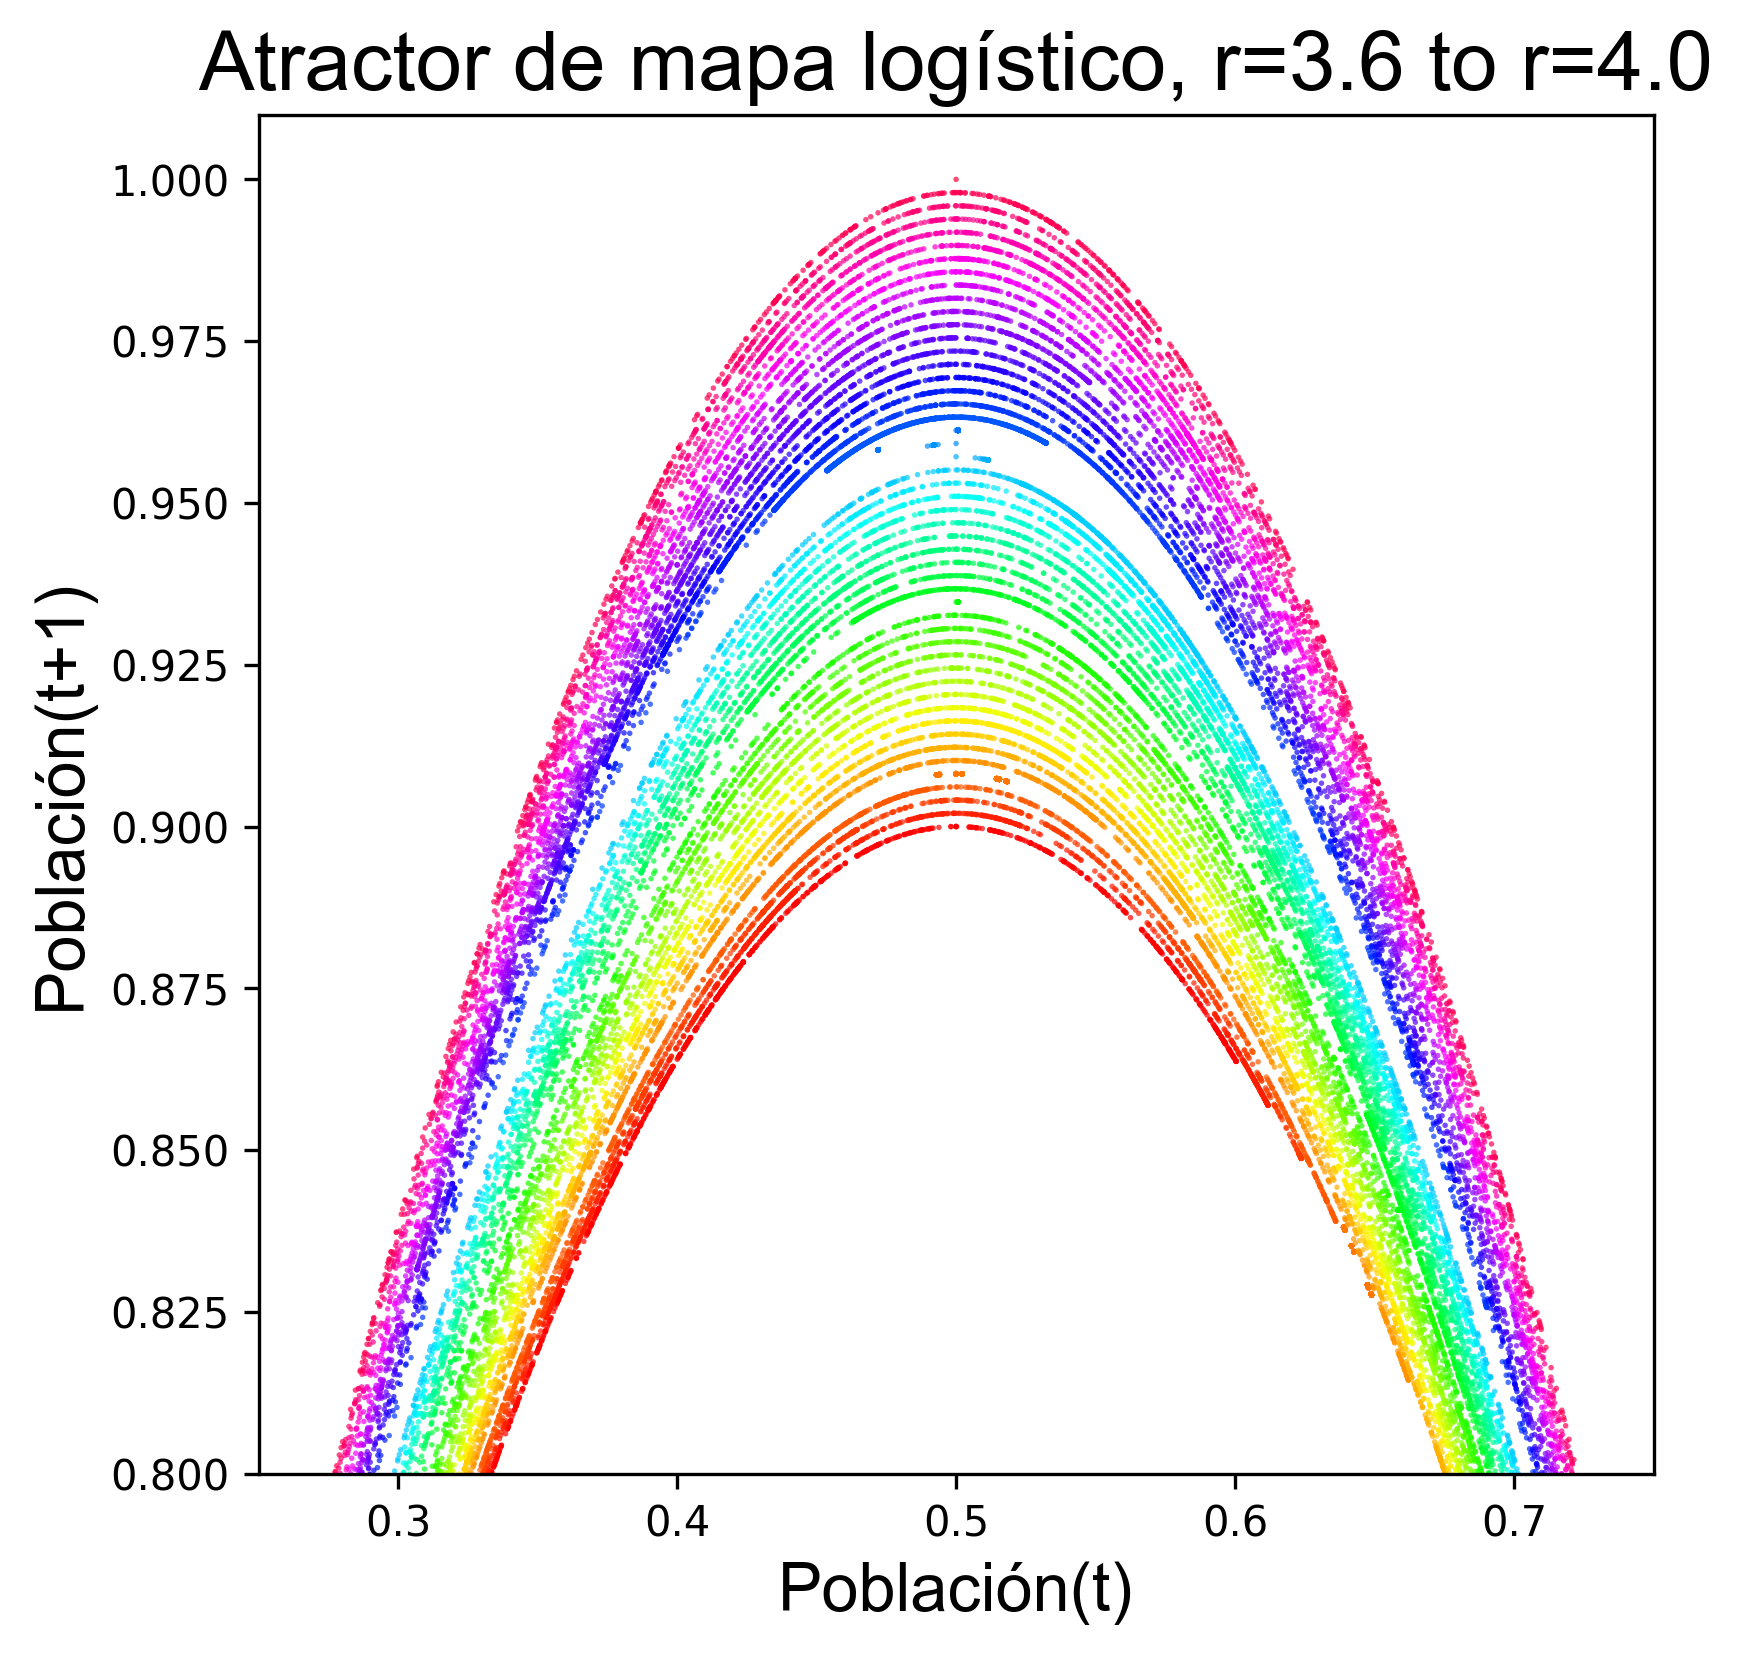
\includegraphics[height=6cm, width=7.5cm]{10}
\end{center}

La gráfica de la izquierda representa una parábola formada por un parámetro de tasa de crecimiento de 3.9. La gráfica de la derecha muestra 50 parámetros de tasas de crecimiento diferentes entre 3.6 y 4.0. Dichos rangos son en los que el mapa logístico se comporta de manera caótica. 
\\


Estos diagramas de fases representan el espacio de estado bidimensional: un espacio imaginario que utiliza las variables del sistema como sus dimensiones.

\begin{center}
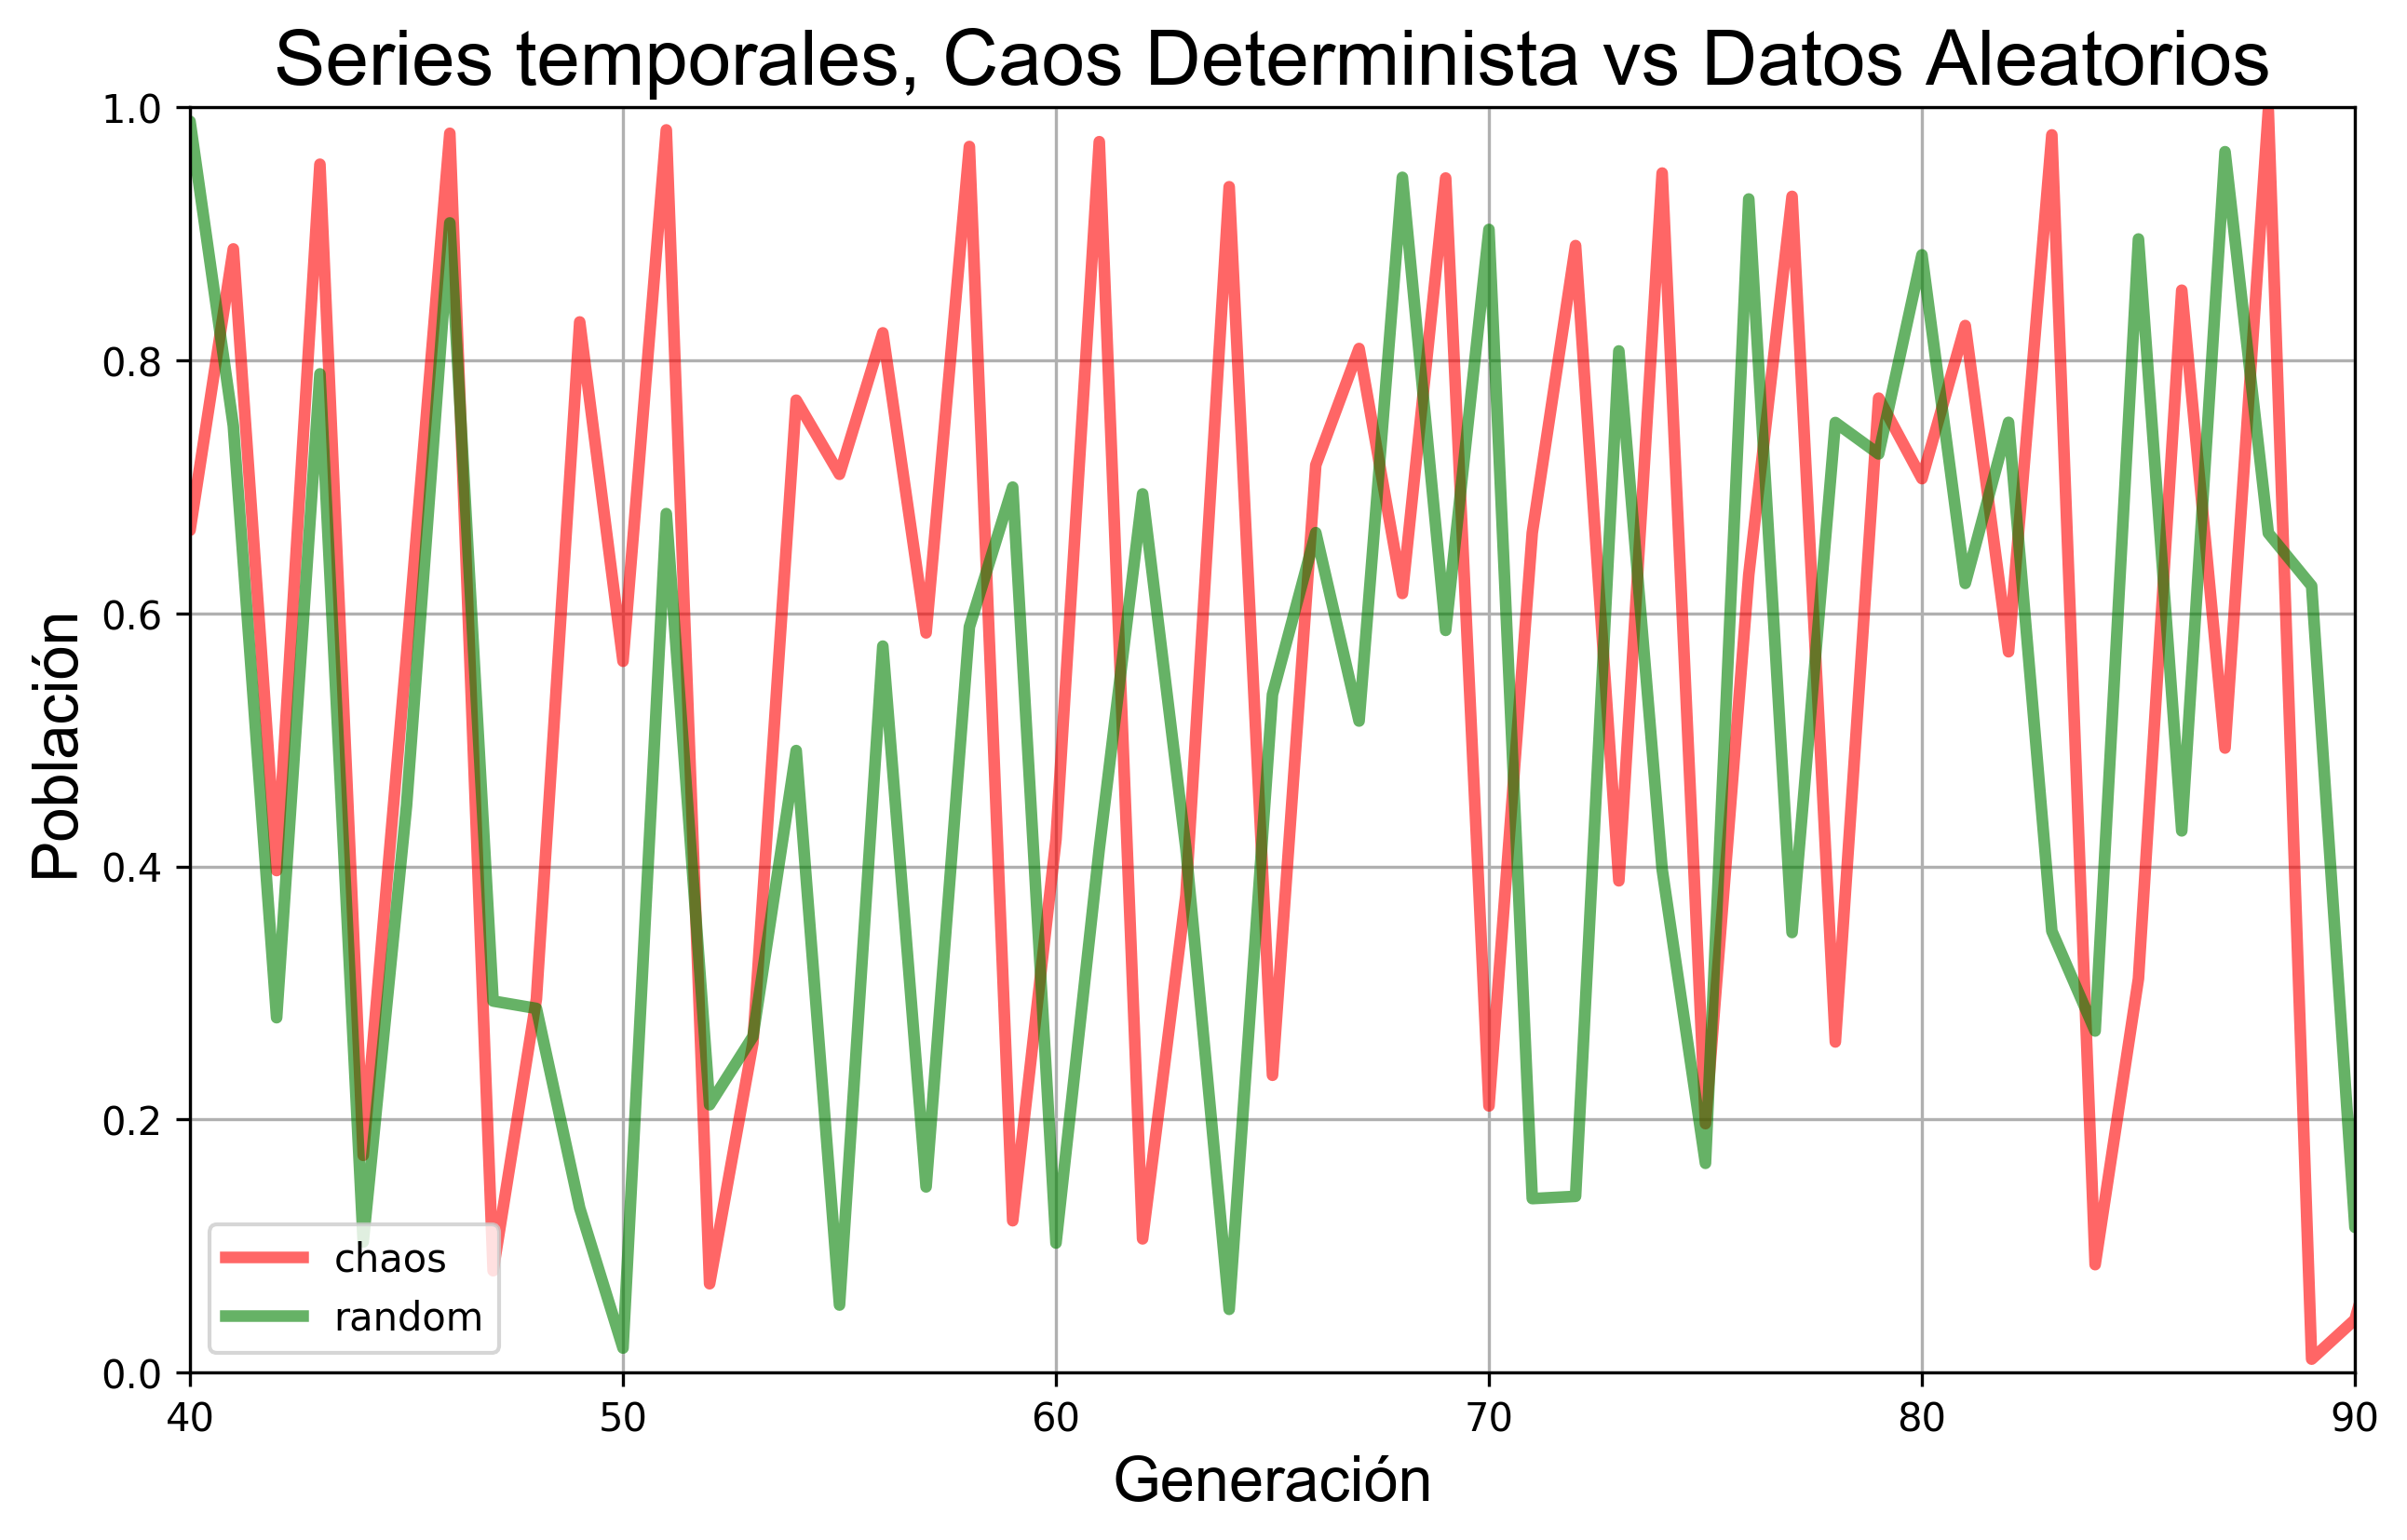
\includegraphics[scale=0.5]{11}
\end{center}

En esta gráficaLa línea verde representa datos aleatorios, pero la línea roja proviene del modelo logístico cuando la tasa de crecimiento se fija en 3,99. Este es un caos determinista, pero es difícil diferenciarlo de la aleatoriedad.

Los mismos dos datos, se presentan en los siguientes diagramas de fase:

\begin{center}
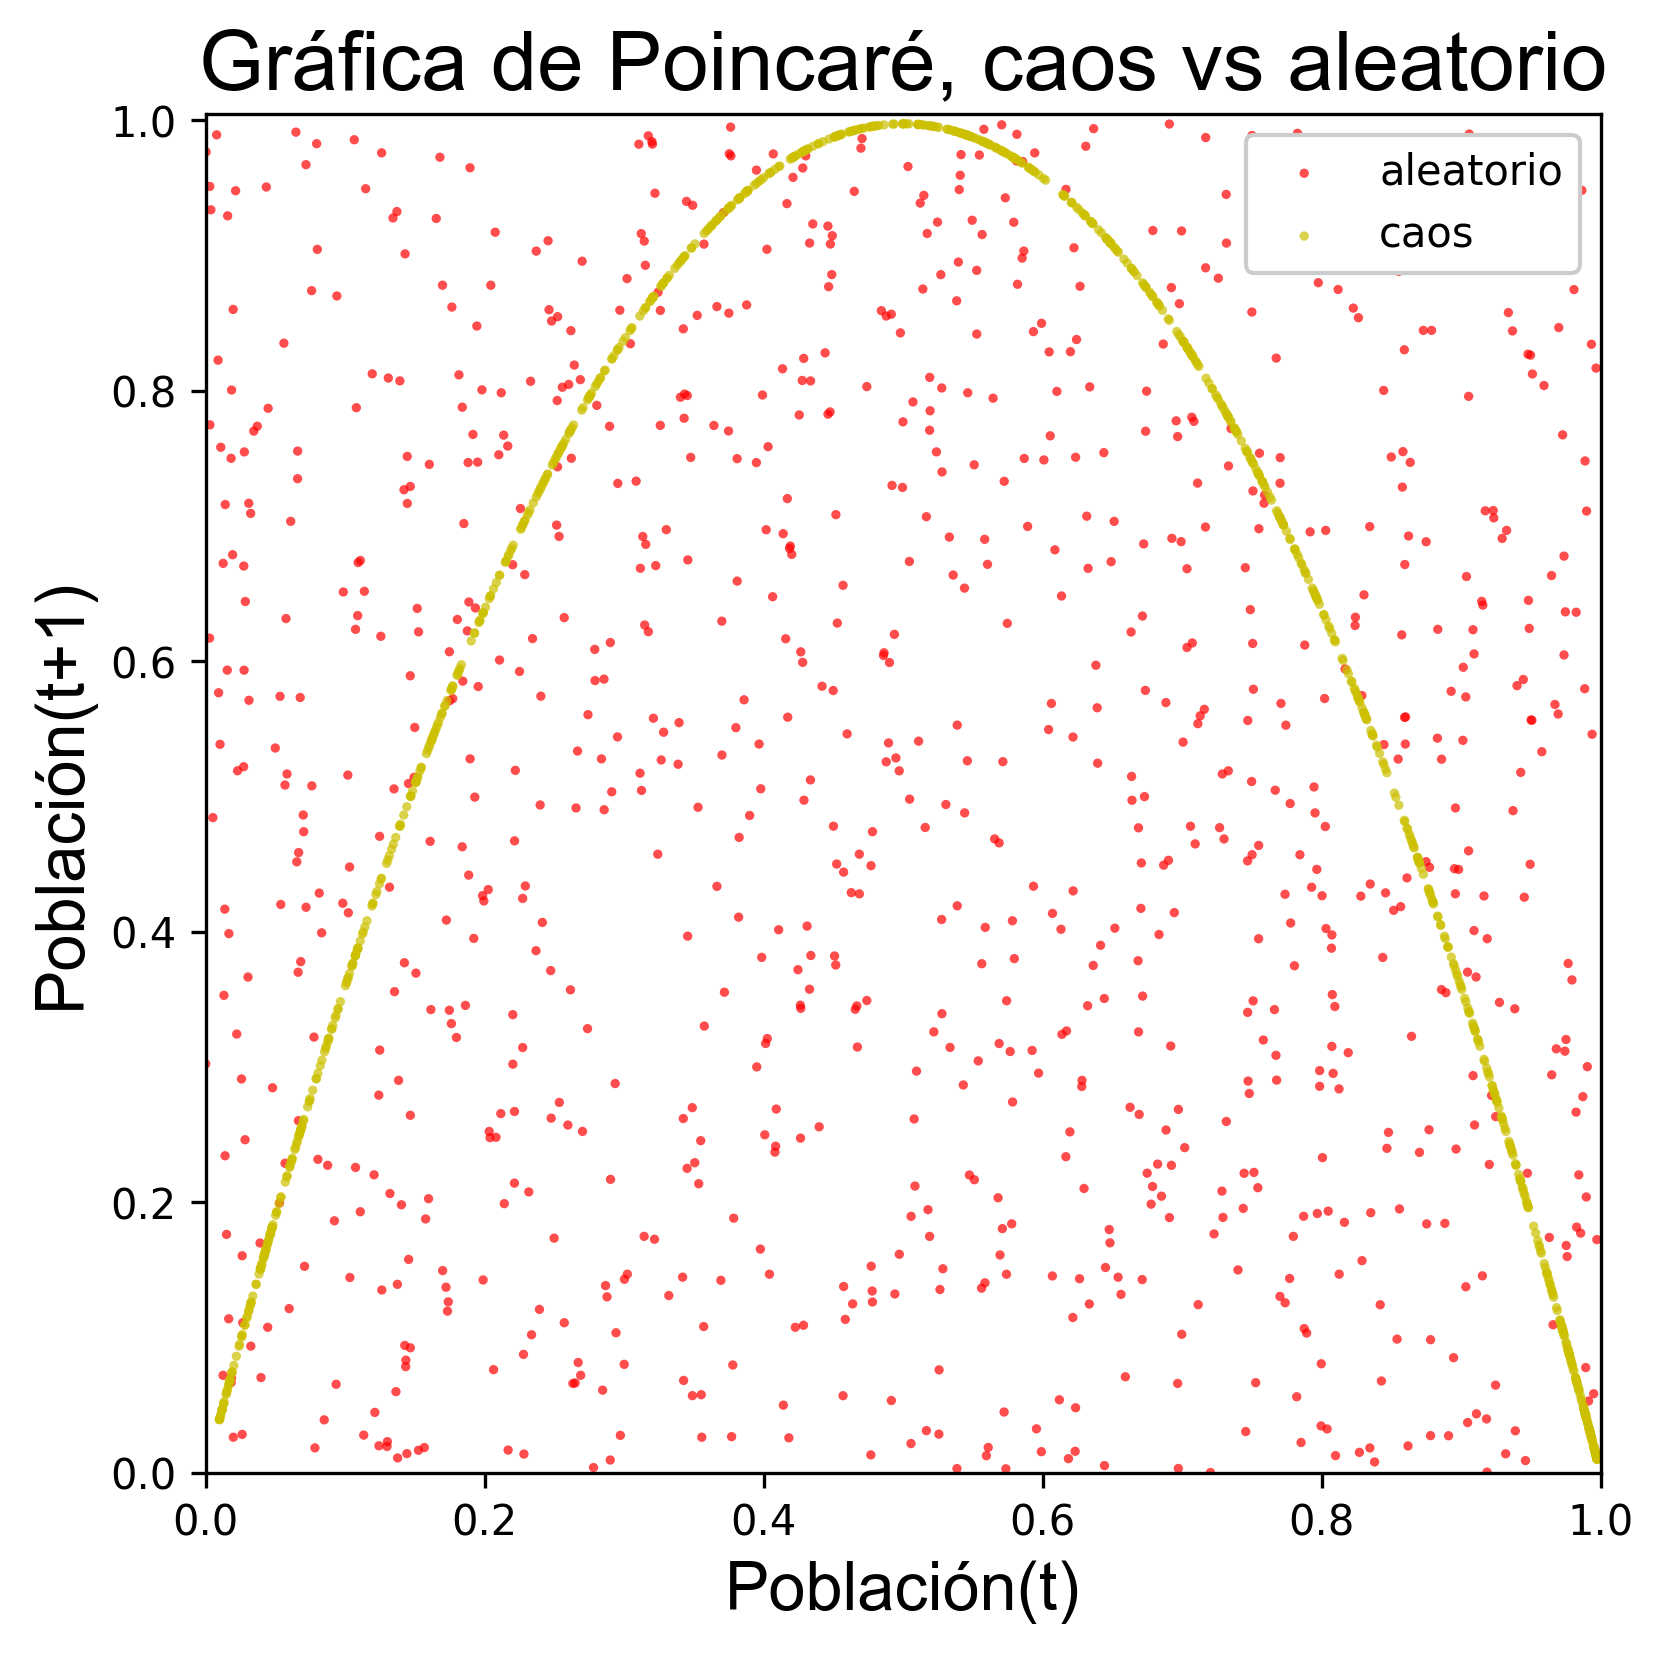
\includegraphics[height=6cm, width=7.5cm]{12}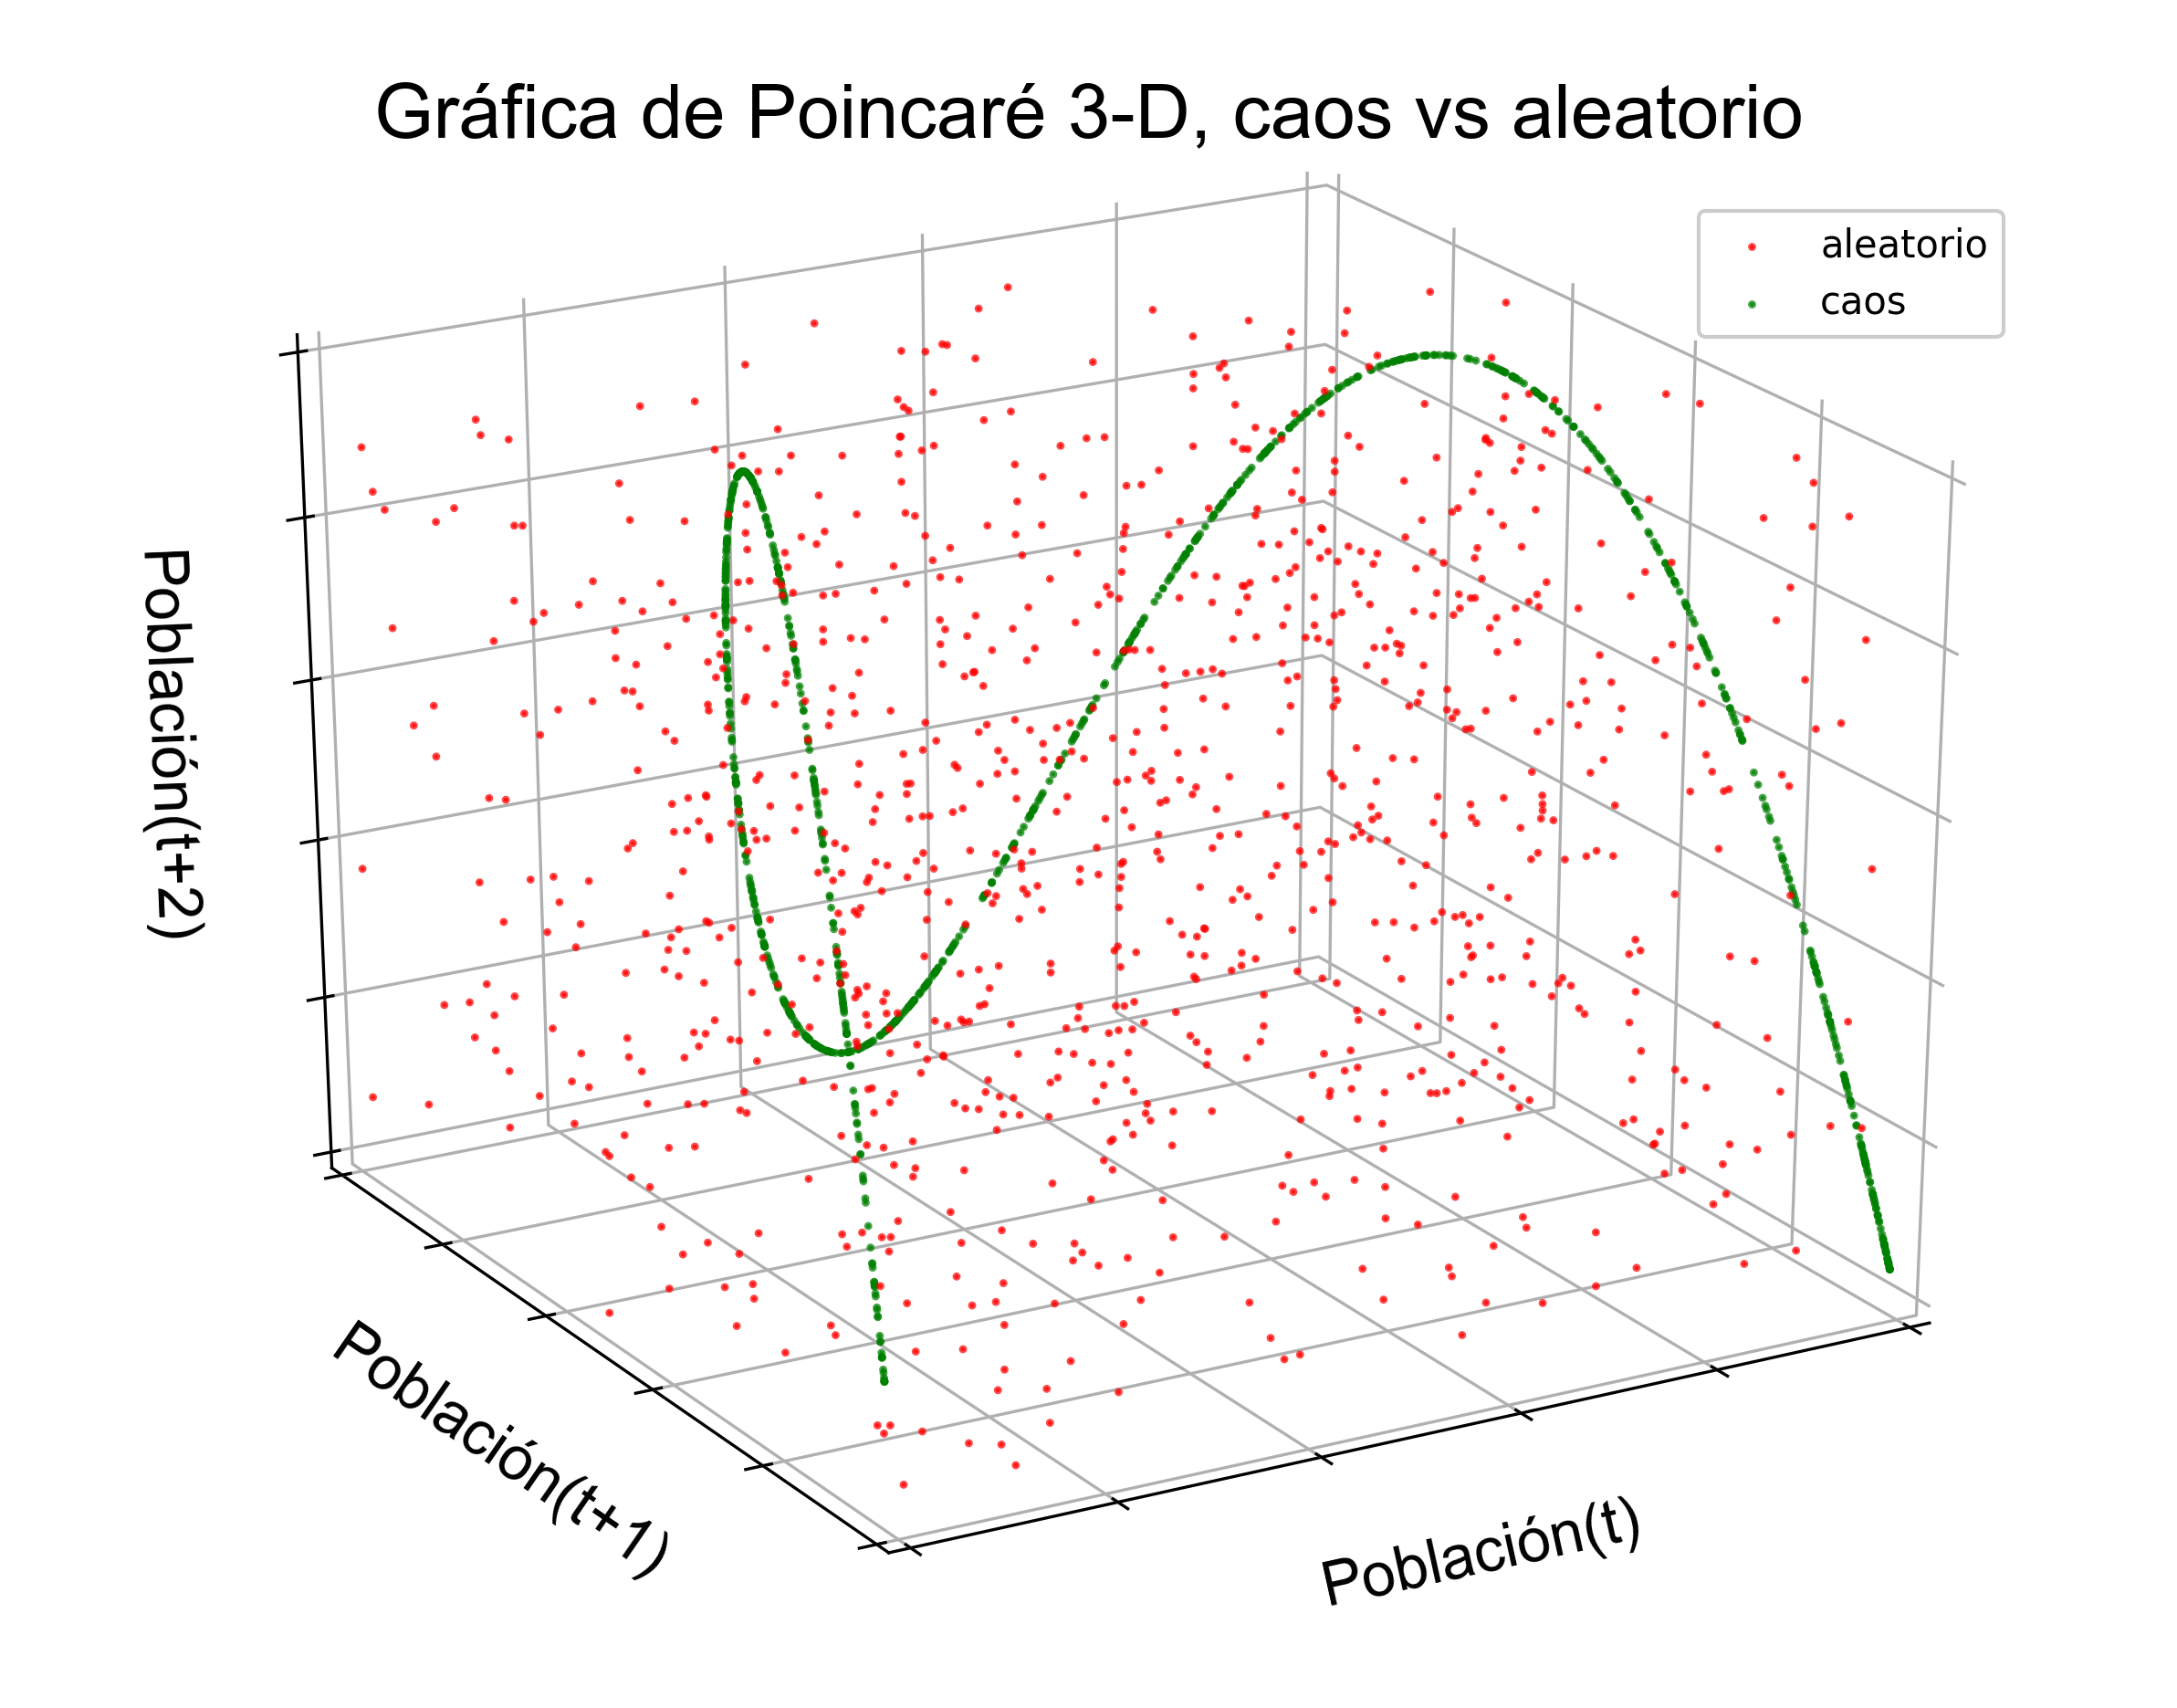
\includegraphics[height=6cm, width=7.5cm]{13}
\end{center}
Los datos aleatorios (en rojo) parecen ser sólo ruido, sin embargo aquí se presenta el sistema caótico (en naranja y verde) constreñido por su extraño atractor.

Lo siguiente es una muestra de la animación obtenida en 3D, la gráfica es del mapa logístico y se puede ver el extraño atractor y su curiosa pero hermosa estructura.
\begin{center}
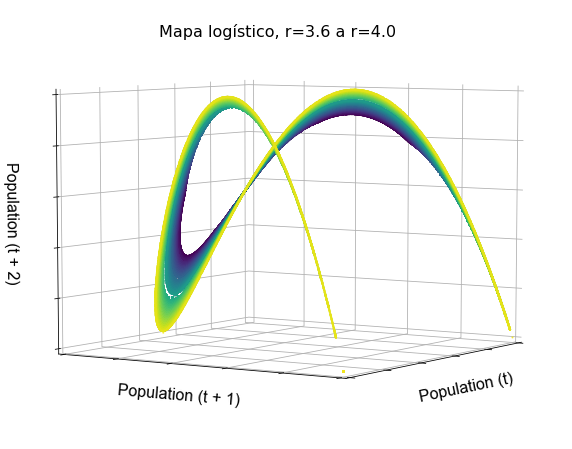
\includegraphics[scale=0.5]{14}
\end{center}

Como ya sabemos, los sistemas caóticos son sensibles a las condiciones iniciales, aquí se presenta una gráfica de mapa logístico, dando dos valores iniciales a la población.

\begin{center}
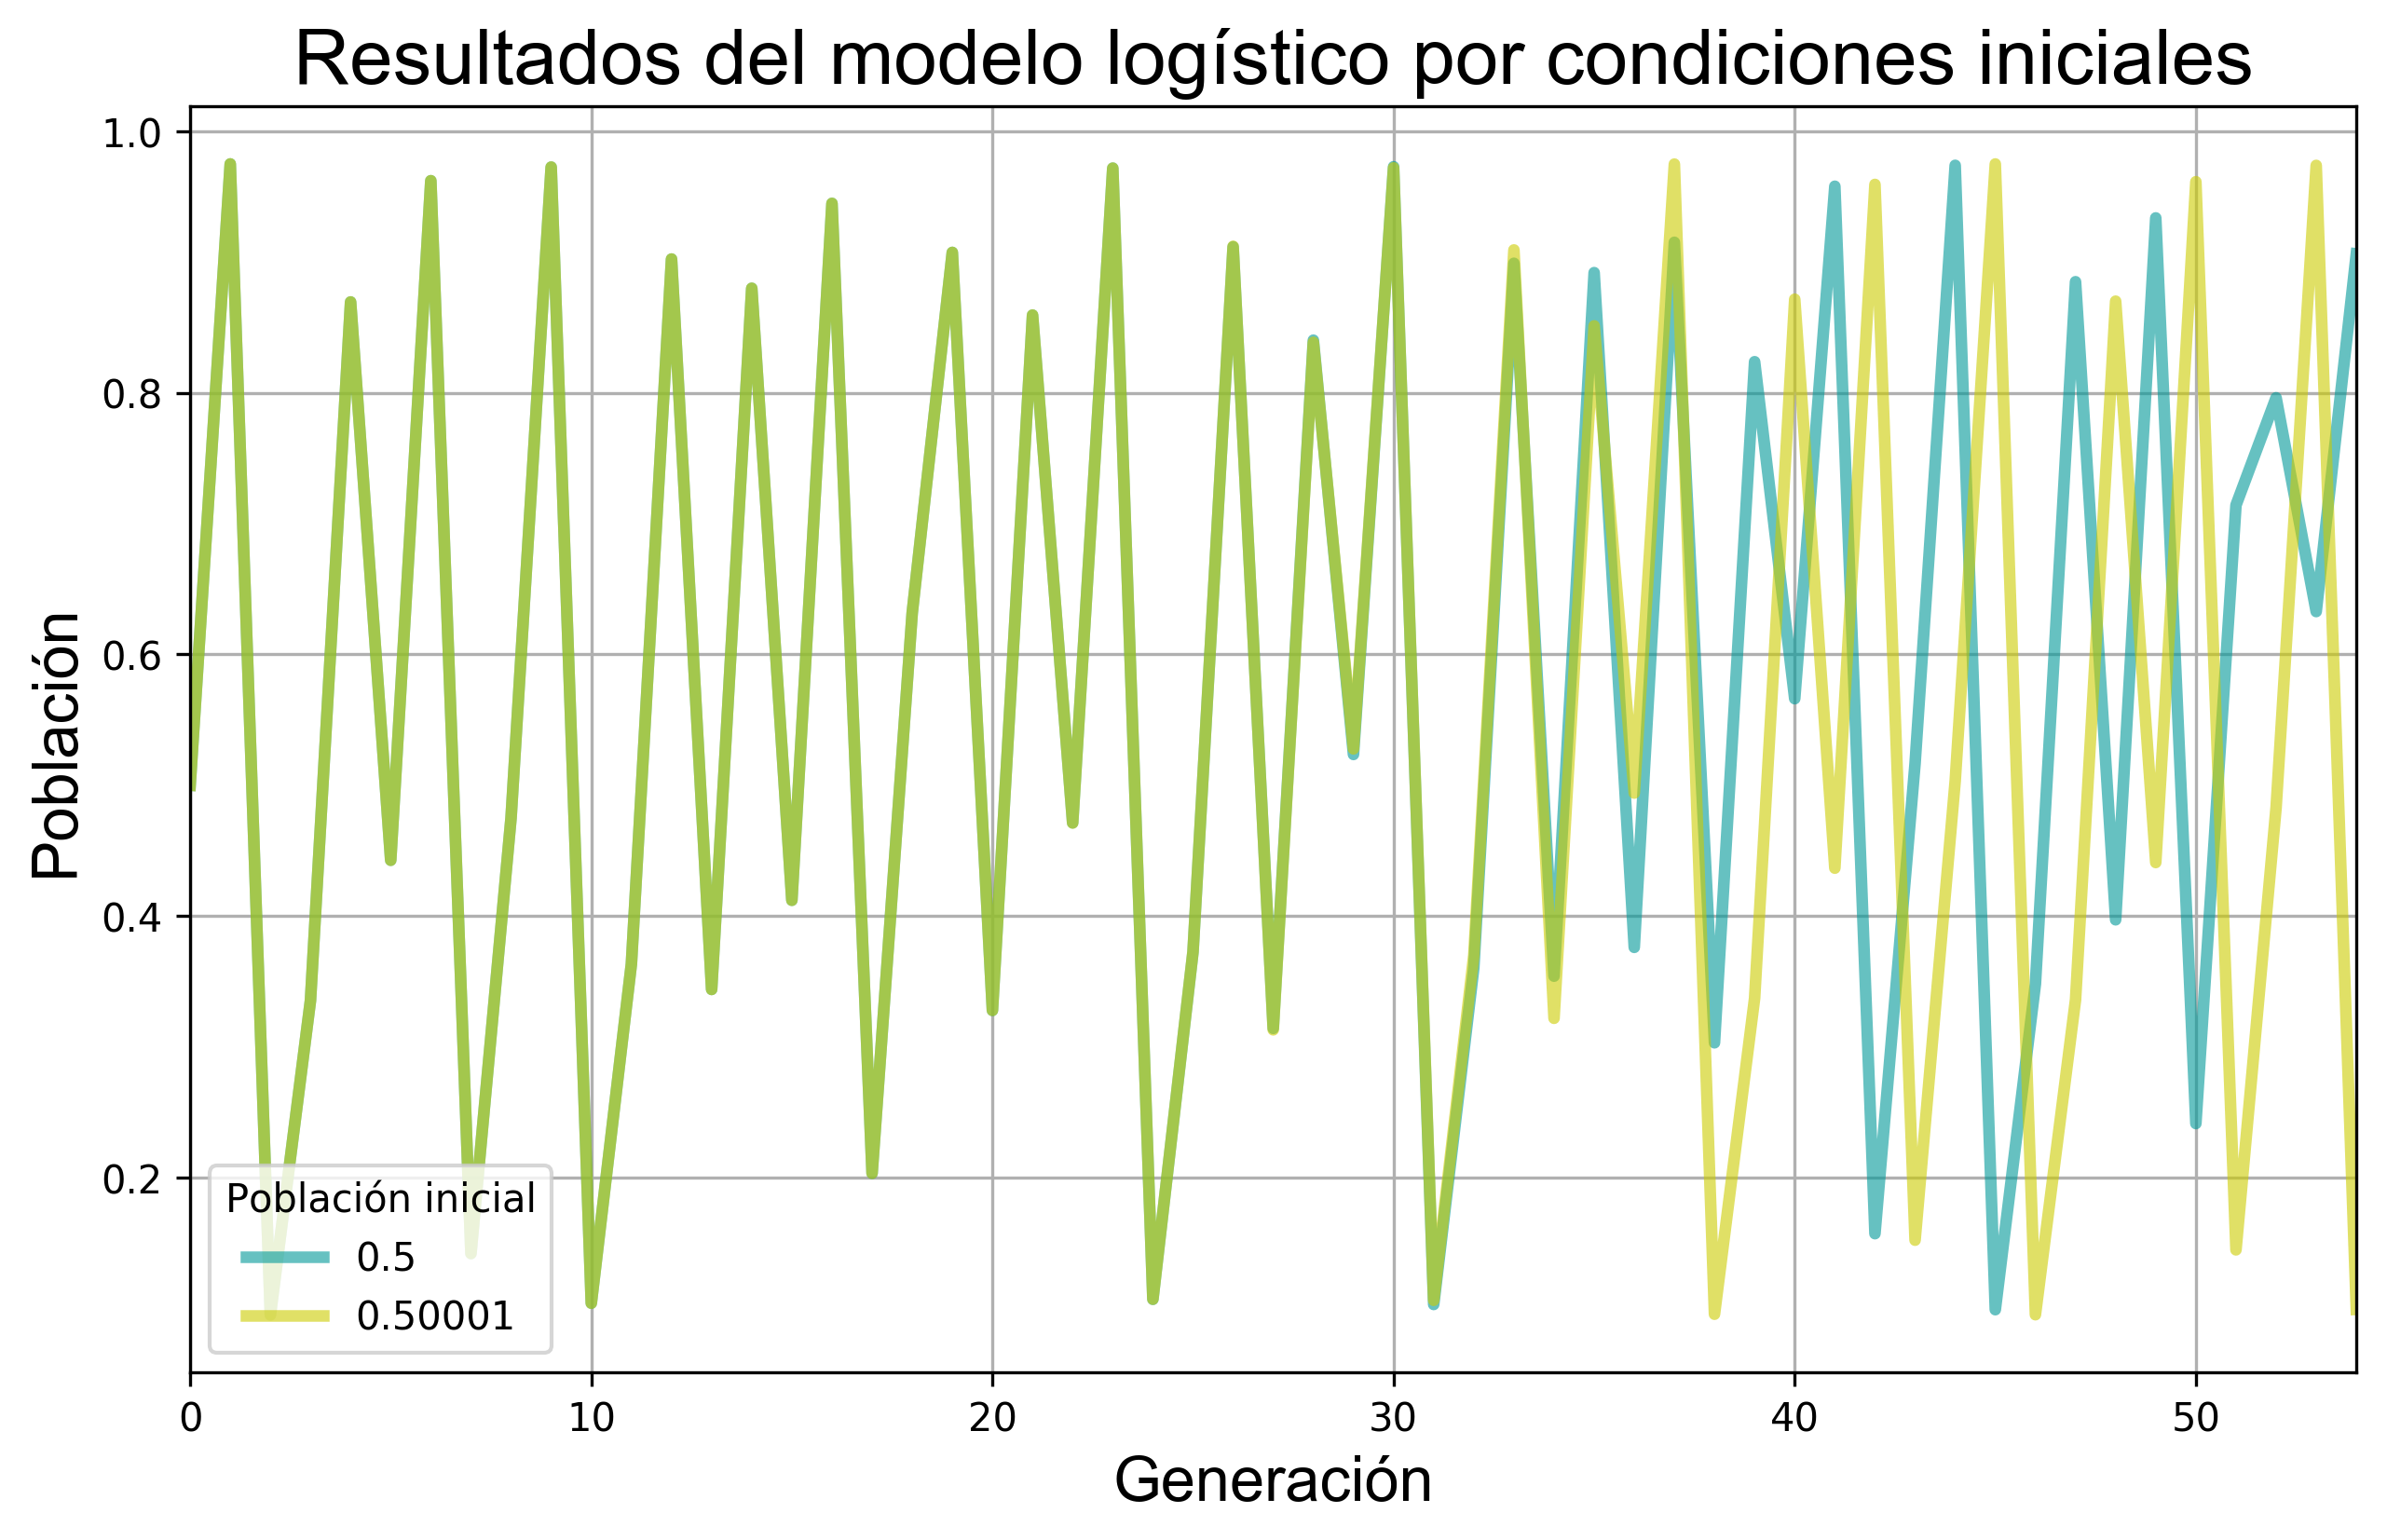
\includegraphics[scale=0.5]{15}
\end{center}

Ambos tienen el mismo parámetro de tasa de crecimiento, 3.9. La línea azul representa un valor poblacional inicial de 0,5. La línea amarilla representa una población inicial de 0.50001. Estas dos condiciones iniciales son demasiado similares entre sí. En consecuencia sus resultados parecen esencialmente idénticos para las primeras 30 generaciones. Después estas comienzan a ser diferentes.

Con esto finalizamos la presentación de las gráficas que aparecen en el artículo de Geoff Boeing.

\section{Conclusión}
Analizar un sistema caótico con diversas gráficas o diagramas es de gran utilidad, pues nos permite ver mejor el comportamiento de dicho sistema, tener varios puntos de vista es importante, pues así no se dejan pasar detalles del comportamiento caótico. En este caso vimos el análisis para la población. Ahora sé que existen muchas herramientas para estudiar los sistemas caóticos y además, ver los atractores extraños de manera animada, brindan una mejor visión del comportamiento de éstos.

\newpage
\renewcommand{\refname}{\section{Referencias}}
\begin{thebibliography}{9}
\bibitem{a1} \textsc{$http://geoffboeing.com/2015/03/chaos-theory-logistic-map/$}

\bibitem{b1} \textsc{$https://github.com/gboeing/pynamical$}

\end{thebibliography}

\end{doublespace}
\end{document}
